
\section{Starve Feeder Development\label{sec:methodology:starveFeeder}}

To automate standardize the starve feeding process, an automatic pellet dispensing starve feeder was developed. This was adapted from an online model and went through various hardware and user interface (UI) iterations.

\subsection{Online Models\label{sec:methodology:starveFeeder:onlineModels}}

It was hypothesized that 3D printing a pellet dispenser would be the ideal development method from a cost and time perspective. Rather than reinventing the wheel, a review of existing 3D printable pellet dispensers was conducted. This was done through online CAD libraries such as Thingiverse and Makerworld with search phrases such as "automatic pellet dispenser" and "automatic fish feeder." Various models were found and one was selected based on applicability, robustness, and ease of implementation. This model is shown in Figure~\ref{fig:methodology:starveFeeder:initialPelletDispenserModel}.

\begin{figure}[h!]
        \centering
        \includegraphics[width=0.7\linewidth]{../figs/methodology/starveFeeder/initial_starve_feeder_design.png}
        \caption{Initial online design of automatic pellet dispenser~\cite{RefWorks:RefID:490-remi-rafael2024pellet}.}
        \label{fig:methodology:starveFeeder:initialPelletDispenserModel}
\end{figure}

\subsection{Finding Materials\label{sec:methodology:starveFeeder:findingMaterials}}

Various materials were needed to create this pellet dispenser. Most of these could be 3D printed, but some had to be either bought or sourced through various engineering labs throughout campus. Table~\ref{tab:methodology:starveFeeder:materialsNeeded} details the required materials.

\begin{table}[h!]
        \centering
        \caption{Summary of material sourcing for starve feeder device components.}
        \label{tab:methodology:starveFeeder:materialsNeeded}
        \begin{tabular}{l l}
                \hline
                \textbf{Material}     & \textbf{Sourcing}        \\
                \hline
                Device Body           & 3D Printed (PLA)         \\
                Auger Screw           & 3D Printed (PLA Tough)   \\
                Ball Bearings         & Labs or 3D Printed (PLA) \\
                Gearbox               & Labs or 3D Printed (PLA) \\
                Drive Belt            & 3D Printed (TPU)         \\
                Ring Stand            & Labs                     \\
                Nema 23 Stepper Motor & Labs                     \\
                UI Components         & Labs                     \\
                \hline
        \end{tabular}
\end{table}

\subsubsection{3D Printed Bearings\label{sec:methodology:starveFeeder:findingMaterials:3dPrintedBearings}}

608 ball bearings were required to ensure smooth rotation of the internal auger screw. While these are relatively inexpensive, the lead time required to order materials through the department was high. As a result, existing 3D printable models of ball bearings were explored. Multiple were printed with the best based on smoothness of rotation and print quality shown below in Figure~\ref{fig:methodology:starveFeeder:printedBallBearings}.

\begin{figure}[h!]
        \centering
        \includegraphics[width=0.7\linewidth]{../figs/methodology/starveFeeder/3D_printed_ball_bearing.png}
        \caption{3D printed ball bearings~\cite{RefWorks:RefID:491-filou3d2023608}.}
        \label{fig:methodology:starveFeeder:printedBallBearings}
\end{figure}

\subsubsection{3D Printed Drive Belt\label{sec:methodology:starveFeeder:findingMaterials:3dPrintedDriveBelt}}

Based on the model designer's recommendation, the drive belt was initially printed with TPU filament. This allowed the belt to be 3D printed while still being flexible like a rubber belt.

\subsection{Auger Screw Optimization\label{sec:methodology:starveFeeder:augerScrewOptimization}}

The auger screw, while printed with PLA Tough filament, was still prone to breaking. The design and printing parameters had to be optimized to strengthen this load-bearing component.

\subsubsection{3D Printing Orientation\label{sec:methodology:starveFeeder:augerScrewOptimization:3dPrintingOrientation}}

The print orientation of this component directly impacted the overall strength of the device (see ~\fullref{sec:literatureReview:printing:optimalParameters:orientation} for an explanation of this concept).
Because a component experiencing torque will fail first due to shear forces, the print layer direction must be considered. If print layer direction is parallel to the direction of torque force, the part will likely fail in shear. As a result, the strongest screw was printed vertically so that the print layer direction is perpendicular to the direction of force. This is illustrated in Figure~\ref{fig:methodology:starveFeeder:augerScrewPrintOrientation}.

\begin{figure}[h!]
        \centering
        \includegraphics[width=\linewidth]{../figs/methodology/starveFeeder/auger_screw_print_orientation.png}
        \caption{Optimal auger screw print orientation based on layer direction. Force explanation created by ChatGPT (left), BambuStudio print setup with force explanation (right). Adapted from~\cite{RefWorks:RefID:432-hanon2020effect}.}
        \label{fig:methodology:starveFeeder:augerScrewPrintOrientation}
\end{figure}

\subsubsection{Infill Percentage\label{sec:methodology:starveFeeder:augerScrewOptimization:infillPercentage}}

The infill percentage of a 3D printed part can also impact its overall strength (see~\fullref{sec:literatureReview:printing:optimalParameters:infillDensity}).

Due to limited material, the entire screw could not be printed at 100\% infill. As a result, the majority of the screw was printed at 50\% infill and the bottom portion that was prone to snapping was printed at 100\% infill.

\subsection{Gear Selection\label{sec:methodology:starveFeeder:gearSelection}}

While the pellet dispensing CAD file included a large gear, it did not include a gear to attach to the stepper motor. Any stepper motors available across Ohio State University labs did not have a gear attached. As a result, a gear had to either be sourced or 3D printed to connect the drive belt to the stepper motor. The gear of interest is highlighted in Figure~\ref{fig:methodology:starveFeeder:stepperMotorGear}.

\begin{figure}[h!]
        \centering
        \includegraphics[width=0.5\linewidth]{../figs/methodology/starveFeeder/stepper_motor_gear.png}
        \caption{Required stepper motor gear (circled in yellow and red)~\cite{RefWorks:RefID:490-remi-rafael2024pellet}.}
        \label{fig:methodology:starveFeeder:stepperMotorGear}
\end{figure}

\subsubsection{Initial Guess and Check Approach\label{sec:methodology:starveFeeder:gearSelection:initialGuessAndCheck}}
% a.	Tried lots of gears to see what fit on the stepper motor best
While a properly sized metal gear could be ordered, the lead time of placing an order through the proper departmental channels was high. As a result, an attempt was made to 3D print a stepper motor gear.

Multiple gear models were found online through CAD libraries like Thingiverse or Makerworld. It was unclear from these models what belt dimensions they were designed for, which led to many models being printed in a "guess and check" approach. Metal gears across various labs at Ohio State University were also trialed throughout this process. Some of these tested gears are shown below in Figure~\ref{fig:methodology:starveFeeder:guessAndCheckGears}.

\begin{figure}[h!]
        \centering
        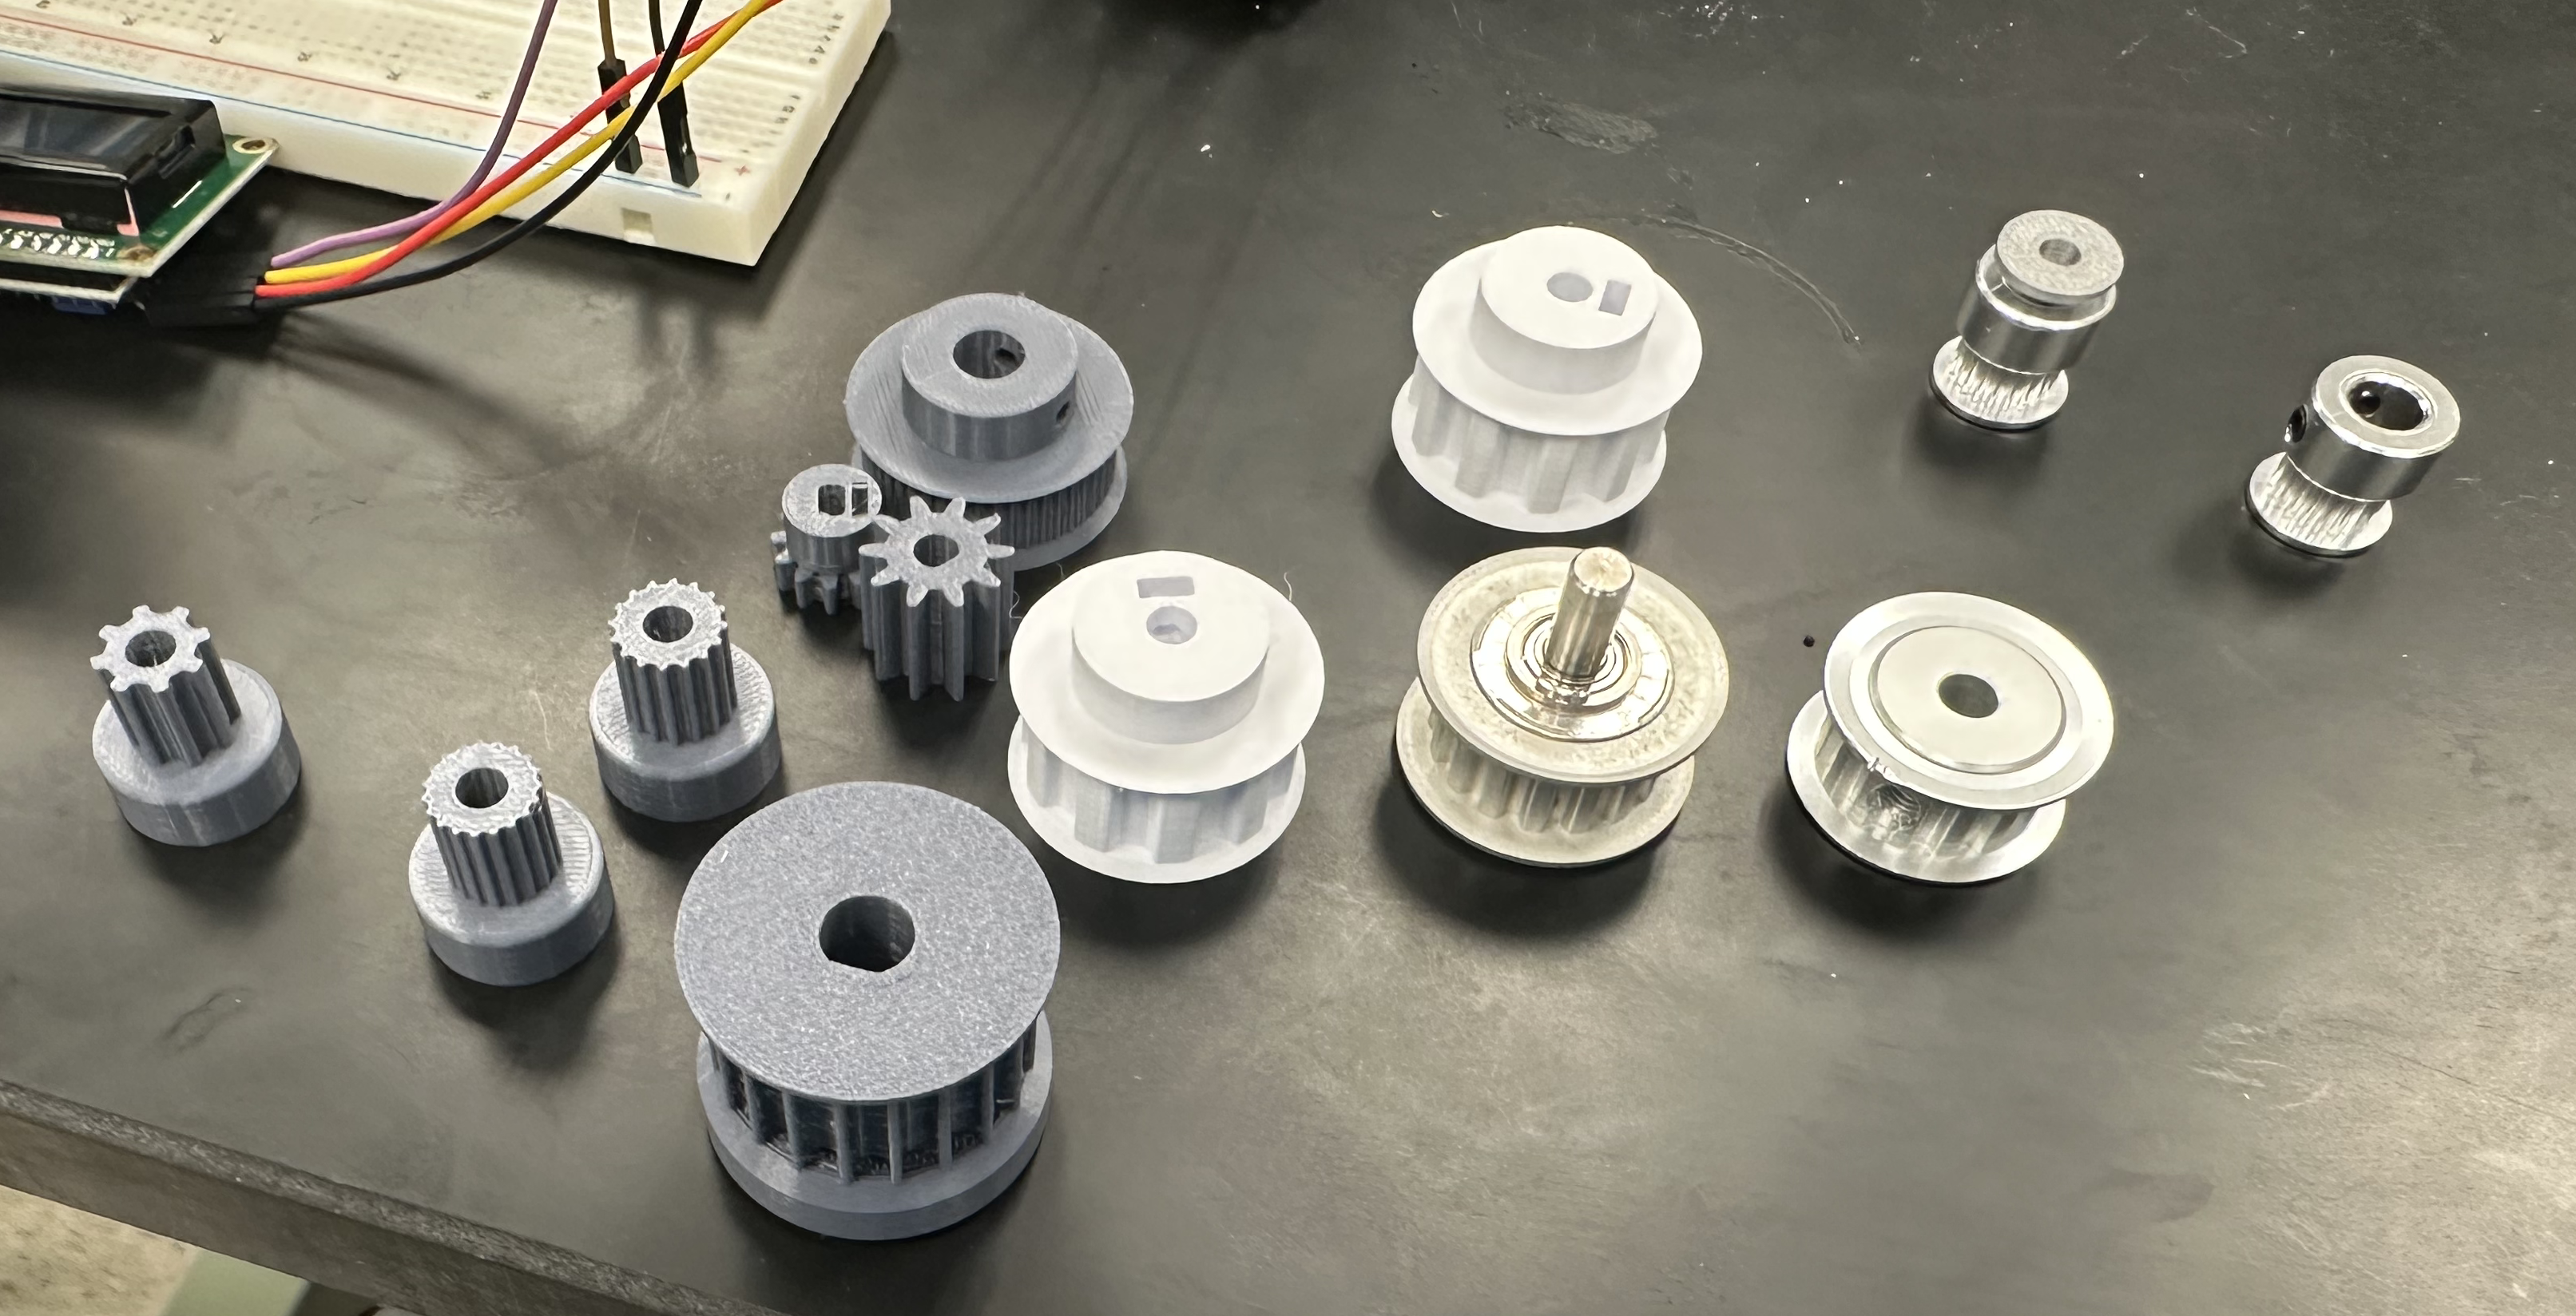
\includegraphics[width=0.5\linewidth]{../figs/methodology/starveFeeder/stepper_motor_gear_attempts.png}
        \caption{Multiple 3D printed gear attempts to interface with stepper motor.}
        \label{fig:methodology:starveFeeder:guessAndCheckGears}
\end{figure}

None of these models fit well enough on the stepper motor to support belt movement. Set screws and model adjustments were also used to try and make these gears more usable.

\subsubsection{Parametric Gear Model\label{sec:methodology:starveFeeder:gearSelection:parametricGearModel}}

A parametric gear modeling tool was found to create gears to exactly match desired sizes and specifications~\cite{RefWorks:RefID:492-koolmgear}. This model allowed for the generation of a usable gear that fit the stepper motor and drive system properly. The specifications for this model are detailed in~\autoref{tab:methodology:starveFeeder:gearSpecs}.

\begin{table}[h]
        \centering
        \caption{Complete Parametric Gear Specifications}
        \label{tab:methodology:starveFeeder:gearSpecs}

        \begin{subtable}{\textwidth}
                \centering
                \caption{Basic Parameters}
                \label{tab:gear_basic}
                \begin{tabular}{cccccc}
                        \hline
                        \textbf{Print Number} & \textbf{Type} & \textbf{Teeth} & \textbf{Width (mm)} & \textbf{Pitch} & \textbf{Bore Type} \\
                        \hline
                        3                     & T5            & 16             & 10                  & 0              & D                  \\
                        \hline
                \end{tabular}
        \end{subtable}

        \vspace{1em}

        \begin{subtable}{\textwidth}
                \centering
                \caption{Dimensional Parameters}
                \label{tab:gear_dimensions}
                \begin{tabular}{cccccc}
                        \hline
                        \textbf{Bore Size} & \textbf{Bore Chamfer} & \textbf{Hub Diameter} & \textbf{Hub Height} & \textbf{Hub Chamfer} & \textbf{Screw Count} \\
                        \hline
                        7.5                & 0.6                   & 20                    & 10                  & 0.6                  & 1                    \\
                        \hline
                \end{tabular}
        \end{subtable}

        \vspace{1em}

        \begin{subtable}{\textwidth}
                \centering
                \caption{Screw Parameters}
                \label{tab:gear_screws}
                \begin{tabular}{ccc}
                        \hline
                        \textbf{Screw Count} & \textbf{Screw Threads} & \textbf{Screw Type} \\
                        \hline
                        1                    & No                     & M4                  \\
                        \hline
                \end{tabular}
        \end{subtable}

\end{table}

\subsection{Initial Slippage Issues\label{sec:methodology:starveFeeder:initialSlippageIssues}}

The custom-designed 3D printed gear attached to the stepper motor and was able to drive the pellet dispensing system. However, when there was resistance in the system, such as due to a slight clog at the dispensing output, the belt began slipping. Either the 3D printed belt or pulley was unable to handle the spikes in torque that the system would experience.

\subsection{Collaboration with Gear Lab\label{sec:methodology:starveFeeder:gearLabCollaboration}}

As a result of the inherent slippage from a fully 3D printed system, the Gear Lab at The Ohio State University was consulted. The team met with Dr. Isaac Hong, a Research Assistant Professor in the Department of Mechanical and Aerospace Engineering. Since this group's research revolves around gear-driven systems, it was believed that they may have suggestions on how to make the pellet dispensing system more robust.

\subsubsection{Belt Tensioning Options\label{sec:methodology:starveFeeder:gearLabCollaboration:beltTensioningOptions}}

The first suggestion proposed for improving the existing system was to add a belt tensioning component. It was hypothesized that adequately tensioning the belt would resolve the belt slippage issues.

Based on belt tensioning design best practices (see~\fullref{sec:literatureReview:beltTension}), multiple concepts were brainstormed including both inside and outside idler pulleys. Some of this brainstorming is shown below in Figure~\ref{fig:methodology:starveFeeder:beltTensioningBrainstorming}.

\begin{figure}[h!]
        \centering
        \includegraphics[width=0.5\linewidth]{../figs/methodology/starveFeeder/belt_tensioning_brainstorming.png}
        \caption{Various brainstorming concepts for a belt tensioning component.}
        \label{fig:methodology:starveFeeder:beltTensioningBrainstorming}
\end{figure}

Based on space limitations and predicted force/stability requirements, the belt tensioning system selected would be an inside idler pulley that could move in the x and y directions. A high-level version of this is shown below in Figure~\ref{fig:methodology:starveFeeder:beltTensioningWinner}

\begin{figure}[h!]
        \centering
        \includegraphics[width=0.5\linewidth]{../figs/methodology/starveFeeder/belt_tensioning_winner_high_level.png}
        \caption{High level representation of selected belt tensioning concept.}
        \label{fig:methodology:starveFeeder:beltTensioningWinner}
\end{figure}

\subsubsection{Gear System Acquisition\label{sec:methodology:starveFeeder:gearLabCollaboration:gearSystemAcquisition}}

In addition to belt tensioning, the Dr. Hong was able to find an old drivetrain system that was powered by a Nema 23 stepper motor. This system was disassembled and the stepper motor pulley, large gear, and rubber belt was used. These metal, plastic, and rubber components replaced the 3D printed counterparts.

The metal stepper motor pulley and rubber drive belt were able to seamlessly replace the existing components in the system. The large gear that drives the auger screw, however, required modifications to the pellet dispenser (see~\fullref{sec:methodology:starveFeeder:systemReDesign:augerScrewReDesign}).

\subsection{Physical System Re-Design\label{sec:methodology:starveFeeder:physicalSystemReDesign}}

Based on the discussions with Dr. Hong at the Gear Lab, the pellet dispenser system was redesigned to include a belt tensioning component and utilize stronger gear and belt components.

\subsubsection{Belt Tensioning Prototyping\label{sec:methodology:starveFeeder:systemReDesign:beltTensioningPrototyping}}

To begin designing the belt tensioning component, a full SolidWorks assembly was created based on the .STL files provided from the online pellet dispenser model.

An assembly was created to ensure that when designing the belt tensioning part, dimensions would line up well with the existing components.

Small edits were made to the frame mount including adding an extra slot for an additional mounting screw and making the attachment holes to the rest of the dispenser larger. Drawings of the final belt tensioning components can be found in  ~\autoref{chap:appendix:solidworksDrawings}:~\nameref{chap:appendix:solidworksDrawings}.

The final SolidWorks assembly including the belt tensioning components is shown below in Figure~\ref{fig:methodology:starveFeeder:beltTensionerAssembly}.

\begin{figure}[h!]
        \centering
        \includegraphics[width=0.7\linewidth]{../figs/methodology/starveFeeder/pellet_dispenser_assembly_with_belt_tensioner.png}
        \caption{SolidWorks assembly of pellet dispenser with belt tensioning component. Frame mount in red and idler pulley adjuster in blue.}
        \label{fig:methodology:starveFeeder:beltTensionerAssembly}
\end{figure}

\subsubsection{Auger Screw Re-Design\label{sec:methodology:starveFeeder:systemReDesign:augerScrewReDesign}}
% a.	Created connection interface for plastic drive gear from gear lab
% i.	Measurements taken using ImageJ
% b.	Connection fit in gear with a press fit
% c.	Added connection to end of screw in SolidWorks
% i.	Re-printed auger screw with new end connection

The auger screw end was re-designed to attach to a stronger large gear provided by the Gear Lab. This gear had a Double D shaft whereas the initial model was designed for a square interface between the screw and the large gear.

To create this design in a way that properly fits the existing gear, an initial image of the gear with a measurement reference was taken as shown in Figure~\ref{fig:methodology:starveFeeder:largeGearUndimensioned}.

\begin{figure}[h!]
        \centering
        \includegraphics[width=0.7\linewidth]{../figs/methodology/starveFeeder/auger_screw_end_redesign_undimensioned.png}
        \caption{Initial image of large gear with calipers for measurement reference.}
        \label{fig:methodology:starveFeeder:largeGearUndimensioned}
\end{figure}

With this initial image, a software called ImageJ was used to measure the slot dimensions. ImageJ works by marking a reference distance, mapping that to a pixel conversion, and then estimating measurements of lines drawn on a photo. The calipers in the initial photo were used for a reference measurement.

Figure~\ref{fig:methodology:starveFeeder:augerScrewMeasuringAndDesign} shows the measurement process and initial design of the attachment piece.

\begin{figure}[h!]
        \centering
        \includegraphics[width=0.7\linewidth]{../figs/methodology/starveFeeder/auger_screw_end_redesign_planning.png}
        \caption{Measurement of large gear using ImageJ (left) and initial design of attachment piece (right).}
        \label{fig:methodology:starveFeeder:augerScrewMeasuringAndDesign}
\end{figure}

Based on these measurements, an attachment piece was created in SolidWorks. This was first printed alone to ensure the estimated dimensions properly aligned with the physical gear. Once it was confirmed that the attachment piece was properly dimensioned, it was attached to the end of the auger screw through a SolidWorks assembly. This combined part was then printed so the auger screw could smoothly attach to the new large gear. The printing modeling of these components is shown below in Figure~\ref{fig:methodology:starveFeeder:augerScrewFinalAttachment}.

\begin{figure}[h!]
        \centering
        \includegraphics[width=0.7\linewidth]{../figs/methodology/starveFeeder/auger_screw_end_redesign_final.png}
        \caption{Auger screw attachment piece (left) and combined screw with attachment (right).}
        \label{fig:methodology:starveFeeder:augerScrewFinalAttachment}
\end{figure}

\subsection{Logic Controls\label{sec:methodology:starveFeeder:logicControls}}

Various Arduino-controlled systems were developed to control the pellet dispenser. Initial iterations used physical components such as a keypad and LCD whereas updated designs relied on a Graphical User Interface (GUI).

\subsubsection{Calibration Method\label{sec:methodology:starveFeeder:logicControls:calibrationMethod}}

To determine how many pellets to pour at a given time, a calibration method was developed. This turned the motor a set number of steps. The user then input how much material in grams this output, and the system would perform a conversion from steps to grams as shown in Equation~\eqref{eq:starveFeederCalibration}.

\begin{equation}
        Pour Steps = \frac{Calibration Steps}{Calibration Weight (g)} * Pour Weight (g)
        \label{eq:starveFeederCalibration}
\end{equation}

\subsection{User Interface\label{sec:methodology:starveFeeder:userInterface}}

The user interface for this device began as a rudimentary component-based control system and advanced to serial-monitor and eventually GUI-based controls.

\subsubsection{LCD and Keypad Control\label{sec:methodology:starveFeeder:userInterface:lcdAndKeypadControl}}

The first iteration of user interface with this device was controlled by an Arduino Uno with a keypad and 16x2 LCD screen connected. Although this design is not space-efficient or sleek, it was chosen to be able to quickly develop and iterate on the functionality of the system.

Instructions on the LCD screen would guide the user through entering and measuring all parameters. This also had failsafes built in to allow the user to go back or re-enter/re-measure values. A home/menu screen with custom icons was made as a central point once the system was running.

Figure~\ref{fig:methodology:starveFeeder:keypadGUI} shows some of the screens and steps for running this keypad-based system. Figure~\ref{fig:methodology:starveFeeder:keypadVersionAssembled} illustrates how the assembled system looks from the outside.

\begin{figure}[h!]
        \centering
        \includegraphics[width=\linewidth]{../figs/methodology/starveFeeder/pellet_dispenser_keypad_gui.png}
        \caption{GUI for keypad and LCD based pellet dispenser (V1).}
        \label{fig:methodology:starveFeeder:keypadGUI}
\end{figure}

\begin{figure}[h!]
        \centering
        \includegraphics[width=0.7\linewidth]{../figs/methodology/starveFeeder/pellet_dispenser_keypad_interface_assembled.png}
        \caption{Assembled keypad-based pellet dispenser.}
        \label{fig:methodology:starveFeeder:keypadVersionAssembled}
\end{figure}

\subsubsection{Conversion to Serial Input\label{sec:methodology:starveFeeder:userInterface:conversionToSerialInput}}

Once the system was operating smoothly, the design and usability were addressed. While the LCD/keypad-based interactions accounted for all steps and failsafes, it was a slow process to enter each number and response on a keypad.

As a result, the Arduino code was adjusted to allow for serial monitor input. With this functionality, users could enter variables and fully control the system directly through the serial monitor.

This code was adjusted with the assistance of ChatGPT and Claude.ai to more quickly implement this functionality.

\subsubsection{Graphical User Interface\label{sec:methodology:starveFeeder:userInterface:graphicalUserInterface}}
% a.	Requires a virtual environment and installing pyserial

Once the system was runnable solely via the serial monitor, the research team decided it would be a straightforward transition to control the entire system through a GUI rather than Arduino IDE. With a GUI, visual elements could be implemented to improve usability of the device. These digital buttons would be directly tied to variable entries making the transition from serial monitor-based control to GUI-based control relatively simple.

To design the GUI, ChatGPT and Claude.ai were utilized. This GUI was run in VSCode on the same computer used to connect to the extruder via DevoVision. Installation of pyserial was required to interact with the Arduino-based code.

With the GUI in place, the keypad was removed from the system.

Figure~\ref{fig:methodology:starveFeeder:pythonGUI} shows the python-based GUI.

\begin{figure}[h!]
        \centering
        \includegraphics[width=0.7\linewidth]{../figs/methodology/starveFeeder/pellet_dispenser_python_gui.png}
        \caption{Python-based GUI for pellet dispenser.}
        \label{fig:methodology:starveFeeder:pythonGUI}
\end{figure}

\subsection{Final System Features\label{sec:methodology:starveFeeder:finalSystemFeatures}}

Various features were designed to make this pellet dispenser user-friendly and portable. These include a simple graphical user interface, countdown timer, multiple pour options, an alarm system, and an adjustable vertical stand.

\subsubsection{Graphical User Interface\label{sec:methodology:starveFeeder:finalSystemFeatures:graphicalUserInterface}}

As mentioned in ~\fullref{sec:methodology:starveFeeder:userInterface:graphicalUserInterface}, a graphical user interface or GUI was developed to make interacting with this system straightforward and efficient.

\subsubsection{LCD Time Display\label{sec:methodology:starveFeeder:finalSystemFeatures:lcdTimeDisplay}}

Although the instructions and interaction are conducted through a GUI rather than an LCD screen in the final design, the LCD screen was kept as a secondary output. Now, the LCD displays a simple countdown until the next pour in case the user can see that more easily than the computer screen.

\subsubsection{Manual Pour Option\label{sec:methodology:starveFeeder:finalSystemFeatures:ManualPourOption}}

A manual pour option was included in the final design. This option can be selected to pour the pre-set pellet weight regardless of whether the automated system is running. This feature was helpful in troubleshooting and also for dispersing pellets immediately if needed.

\subsubsection{Hopper Empty Alarm\label{sec:methodology:starveFeeder:finalSystemFeatures:hopperEmptyAlarm}}

A crucial safety component included in the final design is the "Hopper Empty" alarm. This sounds when the hopper is empty or close to empty. The 3Devo extruder should never be run without steady feed into the barrel, so this alarm ensures pellets are added when necessary. Without this alarm, there is more of a chance that the dispenser will run out of pellets and no material will be fed into the extruder.

The alarm is triggered by logic that subtracts how much material was initially loaded into the hopper from the running total amount of material dispensed through calibrations and pours.

\subsubsection{Adjustable Vertical Stand\label{sec:methodology:starveFeeder:finalSystemFeatures:adjustableStand}}

A vertical adjustable stand was created to maneuver and adjust the pellet dispenser as necessary. The online CAD model of this device utilized a ring stand to hold the pellet dispenser. After searching through various engineering labs, the research team was unable to locate a ring stand. As a result, this structure was created, as shown below in Figure~\ref{fig:methodology:starveFeeder:verticalStand}. Using this stand, the pellet dispenser can be placed on a table or the top of the extruder depending on the experimental setup.

\begin{figure}[h!]
        \centering
        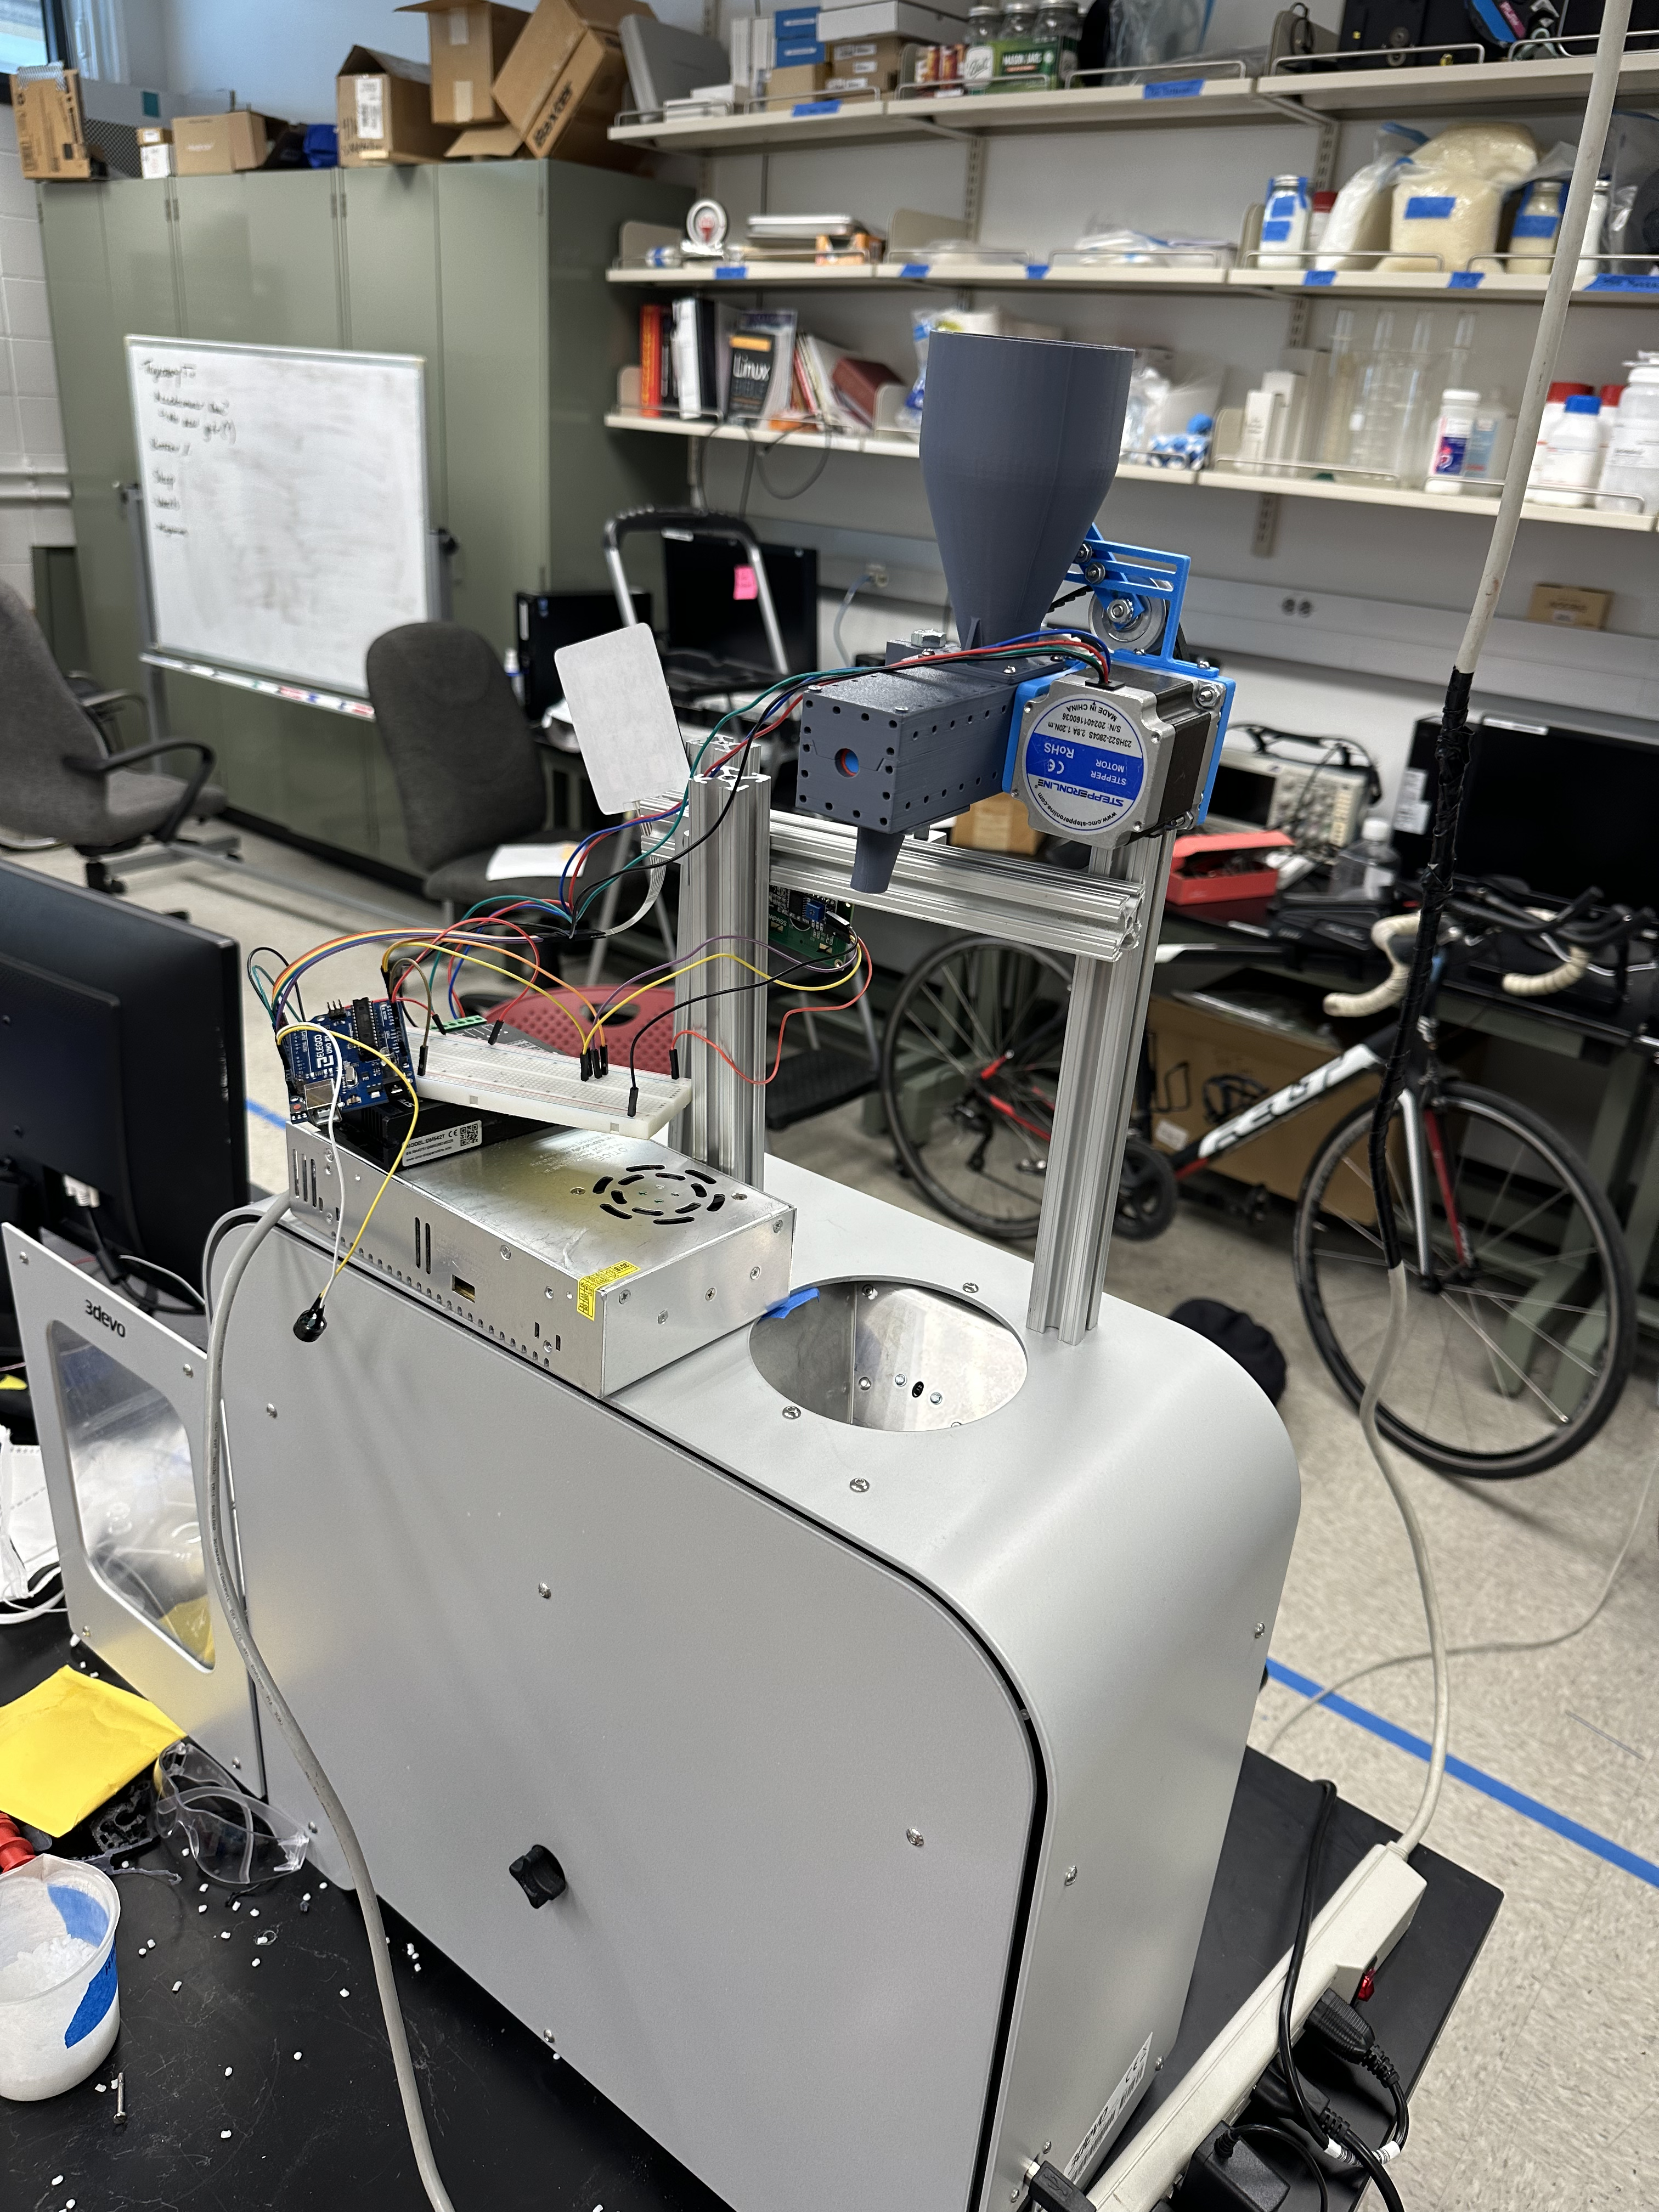
\includegraphics[width=0.4\linewidth]{../figs/methodology/starveFeeder/pellet_dispenser_using_vertical_stand.png}
        \caption{Pellet dispenser atop extruder connected to adjustable vertical stand.}
        \label{fig:methodology:starveFeeder:verticalStand}
\end{figure}

\subsection{Testing Accuracy of Pellet Dispenser\label{sec:methodology:starveFeeder:testingAccuracy}}

Once the starve feeder was operational, testing was conducted to measure the accuracy of the pouring. A desired pour weight of 0.5g, 1.0g, 2.0g, and 5.0g were selected. 20 measurements were taken at each pour level, and each output was weighed to compare the output to the desired weight.

Results and discussion of this testing can be found in ~\fullref{sec:results:starveFeeder} and ~\fullref{sec:discussion:starveFeeder} respectively.
